\chapter*{Conclusion et ANNEXE}

\addcontentsline{toc}{chapter}{Conclusion et ANNEXE}
%\setlength{\parindent}{2cm} 
%\setlength{\parindent}{1cm}
\hspace{0.58cm}

\section {Conclusion}

En conclusion, ce rapport a décrit une méthode de détection de point de rupture pour des lois normales asymétriques, permettant d'obtenir le point de rupture optimal ainsi que les paramètres des lois de part et d'autre du point de rupture. Cette méthode a ensuite été appliquée à des données mensuelles de TER pour différentes régions. \\

L'application s'est révélée plutôt concluante. En effet nous avons obtenus des points de rupture ainsi que des estimations de paramètres de lois cohérents aux données observées.\\

Concernant la correspondance entre droites théoriques et histogrammes nous avons obtenus des résultats plus ou moins satisfaisants selon la série temporelle et la région donnée. Les exemples décevants pourrait avoir plusieurs causes. D'une part, le modèle n'était peut être pas le mieux adapté aux données. D'autre part, l'utilisation de la fonction scipy.minimize peut parfois nous faire atteindre des minimums locaux plutôt que globaux. Il aurait par exemple pû être intéressant de tester la réponse pour différentes valeurs initiales. Mais malheuresement, les temps d'execution longs ont été un frein.

\newpage
\section {ANNEXE}

Imports

\begin{figure}[H]
  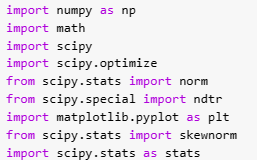
\includegraphics[width=0.5\textwidth]{imports.png}
\end{figure}


\subsection{Code permettant d'estimer les paramètres des lois pour un k donné}

D'abord nous avons défini une fonction retournant la vraisemblance en fonction de l'échantillon, des paramètres des lois et du moment de rupture choisi

\begin{figure}[H]
  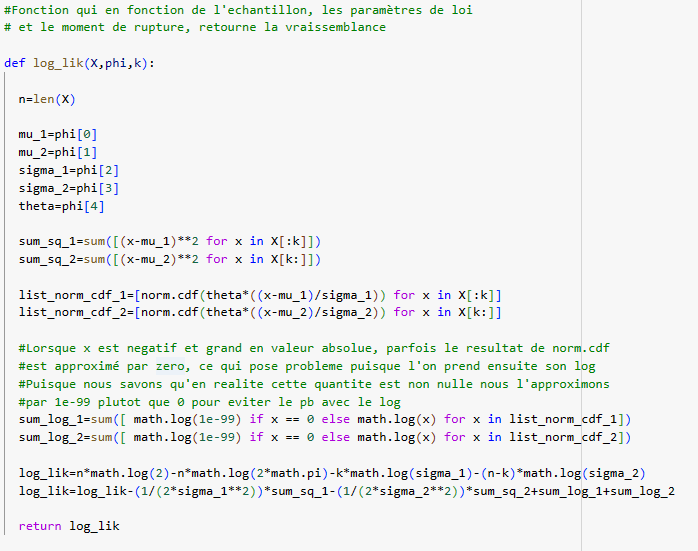
\includegraphics[width=1\textwidth]{ANNEXE_1.png}

\end{figure}

Nous avons ensuite pu définir la fonction renvoyant l'estimation des paramètres par maximisation de la vraisemblance en fonction du point de rupture choisi

\begin{figure}[H]
  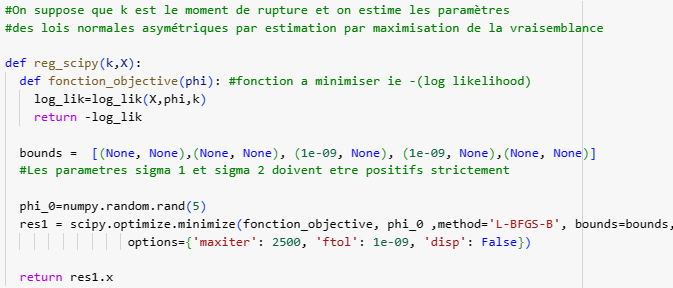
\includegraphics[width=1\textwidth]{ANNEXE_2.png}
\end{figure}

\subsection{Code permettant de trouver le point de rupture optimal}

\begin{figure}[H]
  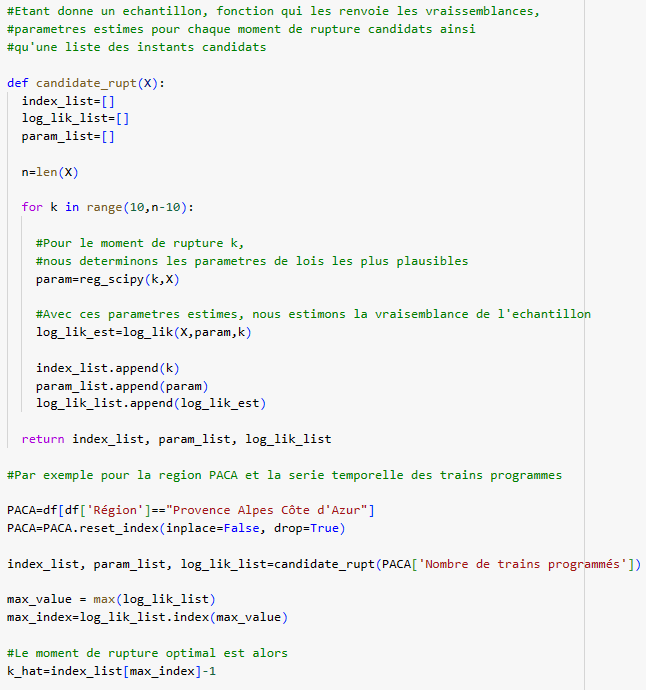
\includegraphics[width=1\textwidth]{ANNEXE_3.png}
\end{figure}

\subsection{Test de Kolmogorov-Smirnov}

\begin{figure}[H]
  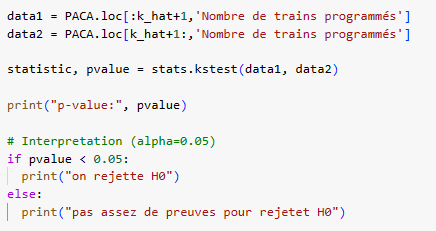
\includegraphics[width=0.7\textwidth]{ANNEXE_4.png}
\end{figure}

Le détail du reste du code se trouve dans le fichier code joint au rapport.
